\documentclass{beamer}
\usetheme{uic}
\usepackage{amsfonts,amsmath,oldgerm,algorithmic,algorithm}
\usepackage[font=small,labelfont=bf]{caption} % Required for specifying captions to tables and figures

\newcommand{\hrefcol}[2]{\textcolor{uihteal}{\href{#1}{#2}}}
\newcommand{\testcolor}[1]{\colorbox{#1}{\textcolor{#1}{test}}~\texttt{#1}}

% Please see Section 18.1 of Beamer User Guide for all the options \usefonttheme provides
\usefonttheme[onlymath]{serif}
% \usefonttheme{serif} % use this if you would like Serif font throughout (and not just for math)

\title{Présentation de soi}
%\titlebackground{images/uic_halls.jpg}
% an asterisk will split the background:
% \titlebackground*{images/uic_seo.jpg}
\titlebackground*{images/Network_Data_Science_and_AI.jpg}
%\subtitle{Using \LaTeX\ to prepare slides}

\author{\href{mailto:haozhang@me.com}{Hao ZHANG}}
\date{\today}

\begin{document}
	\maketitle
	
	% default is no footline, but page numbers are incredibly useful for the audience to ask questions later
	\footlinecolor{uicblue}
	
	\begin{frame}{À propos de moi…}
		Je m'appelle Hao ZHANG,  je suis chinois, j'habite à Paris actuellement…
		\begin{itemize}
			\item En 2022, j'ai terminé mes études de Mastère Spécialisé\textsuperscript{\textregistered} en SMART SYSTEMS \& IoT à CY Tech (anciennement EISTI).
			\item Avant de poursuivre ce Mastère Spécialisé\textsuperscript{\textregistered}, je suis diplômé de l'École d'Ingénieurs Léonard de Vinci (ESILV), spécialité Informatique, Big Data et Objets Connectés (IBO) dans le parcours recherche avec l'option de Data Science.
			\item J'ai deux différentes formations…
		\end{itemize}
	\end{frame}
	
	\begin{chapter}[images/Formations.jpg]{steelgray}{Deux différentes formations}
	\end{chapter}
	
	\begin{frame}[fragile]{Dans le domaine de santé}
		\begin{itemize}[<+->]
			\item J'étais un étudiant en médecine à niveaux de licence.
			\item En 2009, après mon diplôme de licence, j'ai participé à un programme international entre la Chine et la France, donc j'ai eu une chance de faire de simples stages (plutôt comme un observateur) aux hôpitaux parisiens.
			\item Après mon retour, j'ai travaillé dans une entreprise pharmaceutique chinoise, comme un chercheur en analyse stratégique de l'industrie pharmaceutique.
		\end{itemize}
	\end{frame}
	
	\begin{frame}[fragile]{Pourquoi commencer à apprendre la science des données ?}
		\begin{itemize}[<+->]
			\item En raison de mon travail dans cette période, j'ai été exposé à de nombreux travaux d'analyse de données, j'ai progressivement accumulé un fort intérêt pour cet aspect.
			\item J'ai eu des conseils d'un leader respecté de l'industrie.
			\item Enfin, je remarque une énorme opportunité d'unification et de synergie potentielle dans le domaine de la santé avec les technologies de mégadonnées.
		\end{itemize}
	\end{frame}
	
	\begin{chapter}[images/Machine_Learning.jpg]{uicblue}{La commence d'apprendre la science des données}
		\textit{Suivez la tendance et je vais progressivement de plus en plus loin…}
	\end{chapter}
	\themecolor{light}
	
	\begin{frame}[fragile]{L'apprentissage de la science des données et l'IA}
		\begin{itemize}[<+->]
			\item 2015 - 2017 Université de Chongqing, Ingénieur du Technologie Informatique
			\item 2017 - 2020 ESILV, École supérieure d'ingénieurs Léonard-de-Vinci, Informatique, Big Data et Objets Connectés en option de Data Science 
			\item 2020 - 2022 CY Tech (EISTI), Smart Systems \& Internet of Things 
		\end{itemize}
	\end{frame}
	
	\begin{frame}[fragile]{Les stages en France}
		\begin{itemize}
			\item CSTB, Stagiaire en développement de programmes de simulation économique en Python
			\begin{itemize}
				\item Développement d'un programme de simulation économique VBA avec python ;
				\item Optimisation du programme avec vectorisation pour améliorer la vitesse et l'efficacité des calculs.
			\end{itemize}
			\item ELLIADD de l'UFC, Stagiaire en développement d'une ontologie et sa plate-forme sémantique
			\begin{itemize}
				\item Développement d'une ontologie et une base de données graphique (Neo4j) dans le domaine des humanités numériques ;
				\item Développement de services intelligents sur une plate-forme sémantique à partir d'une base de données liée à ontologie.
			\end{itemize}
		\end{itemize}
	\end{frame}
	
	\begin{frame}[fragile]{Mes pratiques d'apprentissage hors ligne (1)}
		\begin{figure}[!htb]
			\minipage{.9\textwidth}
			\centering\includegraphics[width=.85\linewidth]{images/deep_learning_0.png}
			%\caption{A really Awesome Image}\label{fig:awesome_image2}
			\endminipage\hfill
			\minipage{0.1\textwidth}
			\rotatebox{270}{\normalfont\footnotesize{Learning\_Outcomes\_EN/}}
			\rotatebox{270}{\normalfont\footnotesize{Udemy\_Data\_Science\_Courses\_\\}}
			\rotatebox{270}{\normalfont\footnotesize{https://github.com/RaphaelZH/\\}}  
			\endminipage
		\end{figure}
	\end{frame}
	
	\begin{frame}[fragile]{Mes pratiques d'apprentissage hors ligne (2)}
		\begin{figure}[!htb]
			\minipage{0.32\textwidth}
			\centering\includegraphics[width=\linewidth]{images/deep_learning_1.png}
			%\caption{A really Awesome Image}\label{fig:awesome_image1}
			\endminipage\hfill
			\minipage{0.32\textwidth}
			\centering\includegraphics[width=\linewidth]{images/deep_learning_2.png}
			%\caption{A really Awesome Image}\label{fig:awesome_image2}
			\endminipage\hfill
			\minipage{0.32\textwidth}
			\centering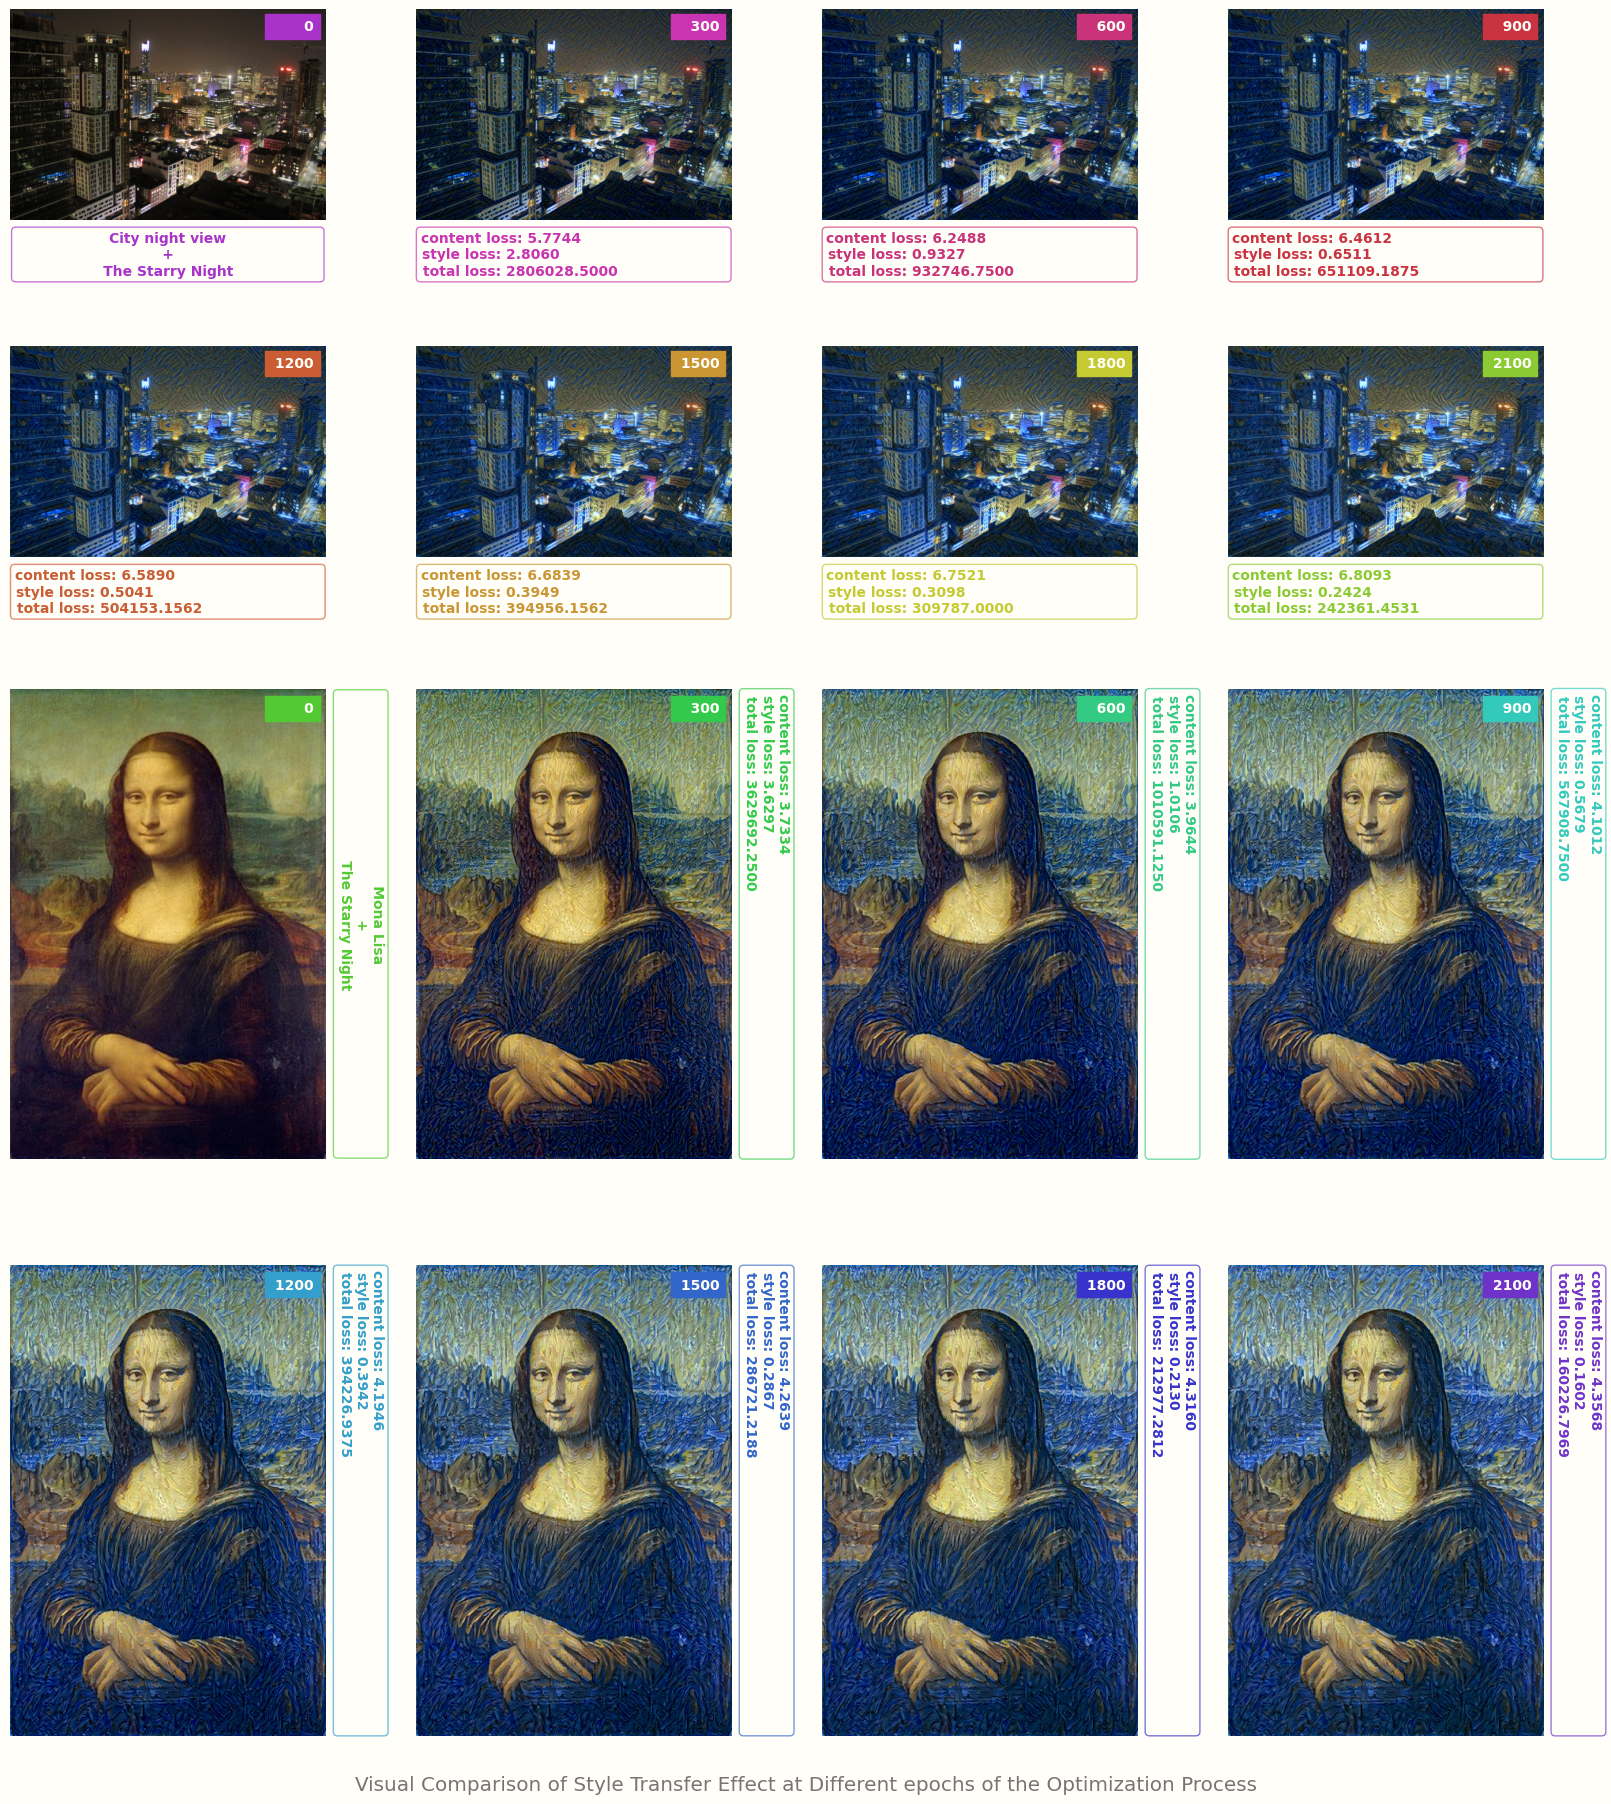
\includegraphics[width=\linewidth]{images/deep_learning_3.png}
			%\caption{A really Awesome Image}\label{fig:awesome_image1}
			\endminipage
		\end{figure}
		\vspace{-.4em}
		\begin{columns}
			\column{0.15\textwidth}
			\column{0.85\textwidth}
			\normalfont\footnotesize{https://github.com/RaphaelZH/Udemy\_Data\_Science\_Courses\_Learning\_Outcomes\_EN/}
		\end{columns}
	\end{frame}
	
	\begin{frame}[fragile]{Mes pratiques d'apprentissage hors ligne (3)}
		\begin{figure}[!htb]
			\vspace{-.25em}
			\minipage{0.34\textwidth}
			\centering\includegraphics[width=\linewidth]{images/deep_learning_4_1.png}
			%\caption{A really Awesome Image}\label{fig:awesome_image2}
			\endminipage\hfill
			\minipage{0.43\textwidth}%
			\centering\includegraphics[width=\linewidth]{images/deep_learning_4_2.png}
			%\caption{A really Awesome Image}\label{fig:awesome_image3}
			\endminipage\hfill
			\minipage{0.1\textwidth}
			\rotatebox{270}{\normalfont\footnotesize{Learning\_Outcomes\_EN/}}
			\rotatebox{270}{\normalfont\footnotesize{Udemy\_Data\_Science\_Courses\_\\}}
			\rotatebox{270}{\normalfont\footnotesize{https://github.com/RaphaelZH/\\}}  
			\endminipage
		\end{figure}
	\end{frame}
	
	\begin{frame}[fragile]{Mes pratiques d'apprentissage hors ligne (4)}
		\begin{figure}[!htb]
			\minipage{.9\textwidth}
			\centering\includegraphics[width=.8\linewidth]{images/dicom.png}
			%\caption{A really Awesome Image}\label{fig:awesome_image2}
			\endminipage\hfill
			\minipage{0.1\textwidth}
			\rotatebox{270}{\normalfont\footnotesize{Learning\_Outcomes\_EN/}}
			\rotatebox{270}{\normalfont\footnotesize{Udemy\_Data\_Science\_Courses\_\\}}
			\rotatebox{270}{\normalfont\footnotesize{https://github.com/RaphaelZH/\\}}  
			\endminipage
		\end{figure}
	\end{frame}
	
	\begin{frame}[fragile]{Mes pratiques d'apprentissage hors ligne (5)}
		\begin{figure}[!htb]
			\vspace{-.25em}
			\minipage{0.33\textwidth}
			\centering\includegraphics[width=\linewidth]{images/deep_learning_5_1_1.png}
			%\caption{A really Awesome Image}\label{fig:awesome_image2}
			\endminipage\hfill
			\minipage{0.33\textwidth}
			\centering\includegraphics[width=\linewidth]{images/deep_learning_5_1_2.png}
			%\caption{A really Awesome Image}\label{fig:awesome_image2}
			\endminipage\hfill
			\minipage{0.3\textwidth}%
			\centering\includegraphics[width=\linewidth]{images/deep_learning_5_2.png}
			%\caption{A really Awesome Image}\label{fig:awesome_image3}
			\endminipage\hfill
			\vspace{.2em}
			\begin{columns}
				\column{0.05\textwidth}
				\column{0.95\textwidth}
				\normalfont\footnotesize{https://github.com/RaphaelZH/Udemy\_Data\_Science\_Courses\_Learning\_Outcomes\_EN/}
			\end{columns}
		\end{figure}
	\end{frame}
	
	\begin{frame}[fragile]{Mes pratiques d'apprentissage hors ligne (6)}
		\begin{figure}[!htb]
			\vspace{-.25em}
			\minipage{0.2\textwidth}
			\endminipage\hfill
			\minipage{0.4\textwidth}
			\centering\includegraphics[width=\linewidth]{images/deep_learning_6_1_1.png}
			%\caption{A really Awesome Image}\label{fig:awesome_image2}
			\endminipage\hfill
			\minipage{0.4\textwidth}%
			\centering\includegraphics[width=\linewidth]{images/deep_learning_6_1_2.png}
			%\caption{A really Awesome Image}\label{fig:awesome_image3}
			\endminipage\hfill
			\vspace{.2em}
			\begin{columns}
				\column{0.05\textwidth}
				\column{0.95\textwidth}
				\normalfont\footnotesize{https://github.com/RaphaelZH/Udemy\_Data\_Science\_Courses\_Learning\_Outcomes\_EN/}
			\end{columns}
		\end{figure}
	\end{frame}
	
	\backmatter
\end{document}
